 \documentclass[10pt]{article}

\usepackage{subeqnarray}
 \usepackage{graphicx}
\usepackage[dvips]{epsfig}
\usepackage{epic}
\DeclareGraphicsRule{.tif}{png}{.png}{`convert #1 `basename #1 .tif`.png}
\usepackage{amssymb}
\usepackage{epstopdf}
\usepackage{amssymb}
\usepackage{amsmath}
\newcommand{\be}{\begin{equation}}
\newcommand{\ee}{\end{equation}}
\newcommand{\bae}{\begin{eqnarray}}
\newcommand{\eae}{\end{eqnarray}}
\newcommand{\bse}{\begin{subeqnarray}}
\newcommand{\ese}{\end{subeqnarray}}
\newcommand{\pade}[2]{\frac{\partial {#1}}{\partial {#2}}}
\newcommand{\pafg}[2]{\frac{\partial #1}{\partial #2}}
\newcommand{\ave}[1]{\langle #1 \rangle }
\newcommand{\eps}{\epsilon}
 \begin{document}
 
\medskip
\centerline{{\LARGE Tutorial 1: Wednesday May 1,   15:15-17:00}}
\vspace{0.5cm}


\noindent {\bf 1. Logistic Regression} \\

\noindent {\bf Notebook: Tutorial1\_1.ipynb} \\

A simple problem to illustrate the use of logistic regression to 
classify Iris flowers is given in the accompanying notebook 
(as was briefly discussed in class on 26/4). Here the sklearn 
package is also used and we will consider only the case of 
two classes (Versicolor, Setosa). \\

\noindent a.   \\
\noindent   Go through the notebook, understand the code 
structure  and identify the hyper parameters.   \\

\noindent b.   \\
\noindent  Study the performance of the classifier on the 
test data for different values of the number of epochs (for
fixed other hyper parameters). \\

\noindent c.   \\
\noindent  Study the performance of the classifier on the 
test data for different values of the regularization
parameter  (for fixed other hyper parameters). \\

\noindent d.   \\
\noindent  Study the performance of the classifier on the 
test data for different values of the learning rate 
parameter  (for fixed other hyper parameters). \\


\noindent {\bf 2. Handwriting Classification with a MLP} \\

\noindent {\bf Notebook: Tutorial1\_2.ipynb} \\

The classification of handwriting digits is one of the classics 
in machine learning. In this tutorial, we will apply a MLP 
on the MNIST data set (see example data in the figure below) 
for this task. The Python  code given is not the most efficient 
one, but it shows explicitly all the  steps involved (including 
the back-propagation algorithm). \\
%
\begin{figure}[htpb]
 \begin{minipage}[t]{\linewidth}
  \centering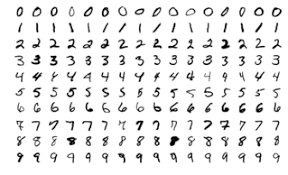
\epsfig{file=figs/mnist.png,width=0.5\linewidth} 
 \end{minipage} \hfill
% \caption{ }
\label{f:F1} 
\end{figure}
%

\noindent a.   \\
\noindent  Go through the notebook, understand the code structure, in 
particular that of the MLP,   and identify the hyper parameters.     \\

\noindent b.   \\
\noindent  For the standard values of the hyper parameters, how many epochs 
are needed to obtain a training error of 5\%?  What is test accuracy in this case?
How would you recognise overfitting in this MLP?  \\

\noindent c.   \\
\noindent  What is the effect of the learning rate on the training error?  
Is there an optimal value? \\ 

\noindent d. \\
\noindent  Study the behaviour of the training error (for a fixed value of 
the number of epochs and the learning rate) versus the number of hidden 
layers in the MLP. Is there an optimal value?  \\ 

\noindent e.  \\
\noindent  How would you determine the global optimum of the hyper parameters?  
{\bf Extra: implement such an optimalization algorithm in the notebook.}  \\ \\  


\end{document}

